\documentclass{article}

\usepackage[utf8]{inputenc}
\usepackage[a4paper]{geometry}
\usepackage[boxed]{algorithm2e}
\usepackage[noend]{algpseudocode}
\usepackage{amsmath}
\usepackage{hyperref}
\usepackage{adjustbox}
\usepackage{xcolor}
\usepackage{listings}
\usepackage{graphicx}
\usepackage{placeins}

\selectcolormodel{gray}

\begin{document}
\vspace*{\fill}
\begin{center}
    {\Huge{Design and implementation of parallel breadth-first search} }\\[2mm]
    \vspace{6.5mm}
    
    {\large \textbf{Project Report}}\\[5pt]
    \vspace{15mm}

    {\large \textbf{Academic year 2020-2021}}\\
    {\large \textit{Submitted for the examination of Parallel and distributed systems: paradigms and models}}\\[5pt]
    \vspace{6.5mm}

    {\large By}\\
    \vspace{3mm}
    {\large\textbf{Giuseppe Grieco}}\\
    {\large g.grieco6@studenti.unipi.it}\\

    \vspace{11mm}
    
\includegraphics[scale=0.07]{./images/logo.png}\\
    \vspace{11mm}

    {\large Department of Computer Science\\
    \textsc{University of Pisa, Italy}}\\
    \vspace{15mm}

    {\large{July, 2021}}
\end{center}
\vspace*{\fill}
\newpage

\tableofcontents


\section{Introduction}
\subsection{Problem statement}
The bread-first search is an algorithm visiting the graph in amplitude. It starts from a node, 
often called the root or source node, and continues visiting all its descendants level
by level, whereas the $i$-th level will contain all the nodes at a distance $i$ from the root.
For each node visited the algorithm checks its label to count the occurrences of the target label.
The assumption underlying all the work is that the input to the problem is a direct and 
acyclic graph. In addition, for the sake of clarity, the notation used is summarized below:
\\

Let $\mathcal{G} = (V, E)$, $|V| = n$ is the number of node and $|E| = m$ is the number of edges. 
For all the node $v \in V$:
\begin{itemize}
    \item $\mathcal{N}(v) = \{u : (u, v) \in E\}$ is the neighborhood of $v$;
    \item $k_{in}(v) = |\{e: e=(u, v) \in E\}|$ is the in-degree of $v$;
    \item $k_{out}(v) = |\mathcal{N}(v)|$ is the out-degree of $v$;
    \item $k(v) = k_{in}(v) + k_{out}(v)$ is the degree of $v$.
    \item $d(u, v)$ is the distance from $u$ to $v$, i.e. the minimum path from $u$ to $v$.
\end{itemize}
Using the node-focus notation above,
 it is possible to define general properties for the graph:
\begin{itemize}
    \item $\bar{k}$ is the average degree;
    \item $\bar{d}$ is the average distance;
    \item $d_{max}$ is the diameter.
\end{itemize}

\subsection{Preliminary analysis}
\subsubsection{Data structure}
Before entering in the algorithmic details let's first introduce the data structure used.
There are many ways to represent a graph among these the main ones are adjacency list and adjacency
matrix. The choices among them is mainly a matter of the usage of the adjacency information and the 
expected nature of the graph. As for every node $v$ of the graph, induced by the root, it will be necessary
to go through each node $u \in \mathcal{N}(v)$, the adjacency list is way more efficient since for each
node $v$ the listing of $\mathcal{N}(v)$ takes a time proportional to $k_{out}(v)$, which is thus optimal.
Moreover, if the expected input of the algorithm are "real" graphs than since they are very sparse, the representation as a adjacency list is way 
more efficient in terms of space complexity.
\\
In particular the presented version represent a graph $G$ as a vector of nodes.
 The node is a pair, the first component is the label of the node, while the second
 component is the adjacency list containing the indices of the nodes in the graph.
\subsubsection{Sequential version}
The sequential version is a straightforward implementation of the problem
description. It makes usage of two vector $F$ and $\hat{F}$: the former is the frontier 
while the latter is used to add new nodes and therefore represents the frontier 
to be used in the next iteration. At the beginning, the algorithm initializes the frontier
with the neighborhood of the source node and marks each child as visited. Then it marks the source node 
as visited and updates occurrences if needed (i.e. if the root has the searched label). After this first phase,
 the algorithm starts the first loop which iterates on each level checking that $F$ is not empty.
 Subsequently, for each level, it goes through each node $v \in F$, updates occurrences if needed and
 then goes through each node $u \in \mathcal{N}(v)$.
 For each node $u$ in the neighborhood, if the node $u$ is not marked as visited, 
 it adds $u$ to $\hat{F}$. After having exhausted all the nodes of $F(i)$, the algorithm
 swaps $F$ with $\hat{F}$ and then clears $\hat{F}$.


\section{Proposed solution}
Before going into the details of the solution, let's describe the graphs 
used for the analysis. The dataset used is a set of synthetic 
graph generated using the Erdos-Renyi model.
Therefore, it is parametric in $p$, whereas $p$ can be interpreted formally as the probability
of attaching a node regardless the previous realizations. On the another hand it
can be seen as the density of the graph. In particular the set used by the experiments
is composed by three different graph of $10000$ nodes with $p = 0.2, 0.4, 0.8$. 
The number of nodes was chosen as a tradeoff on a reasonable size, to evaluate the
goodness of the algorithm and the cost in terms of memory and space required, since
the space and time complexity are $O(n^2)$ which are not negligible.
\subsection{Problem Analysis}
\subsubsection{Completion time}
The sequential algorithm described in section .\ref{sub:seq-version} is an
iterative algorithm with an initialization phase where the $i$-th iteration visits level $i$. The
processing of the $i$-th level requires to go through each node
$v : d(v, s) = i$ and visit its neighborhood.
The time needed to process a node is independent of the
level at which it is visited as it only depends on the size
of its neighborhood. Hence, let the time taken by the node $v$ be denoted 
with $T_v$. Then the time taken by the level $i$ is $T_{L_i} = \sum_{v : d(v, s) = i}T_v$.
Note that different levels require different times depending on the topology of the graph. In particular, the $i$-th level is influenced by the number of nodes at distance $i$ from the root 
and by the size of the neighborhood of these nodes. The completion time of the $i$-th
iteration is given by $T_i = T_{L_i} + T_{swap} + T_{clear}$, i.e. the time taken by the level $i$ plus two additional factor: the former, $T_{swap}$, is the time taken to swap 
$L$ and $\hat{L}$, which is the same for all the iterations since it is a swap of two pointers; the latter, $T_{clear}$, is
time taken by the cleaning of the new $\hat{L}$ so it depends on number of elements.
Let $G$ be the graph induced by the root node then the completion time for the sequential algorithm is:
$$
T_{seq}(G) = T_{init} + \sum^{\bar{d}(G)}_{i=1} T_i \leq  T_{init} + (\bar{d}(G) \cdot max_i \ T_i)
$$

Where $T_{init}$ is the time taken by the
initialization phase, therefore it takes into account: the initialization of the 
vector of visits, the initialization of $F_i$ and $F_{i+1}$, the analysis 
of the root node, the insertion of its neighbors in the frontier and 
the creation of the vector of visits.

There mainly are three kind of possible parallelism:
\begin{enumerate}
    \item The frontier-level: which divides 
    the work required by the computation of the single frontier among the workers;
    \item The neighborhood-level: which divides the work required by the single
    node computation, hence the visit of its neighbors among the workers;
    \item A combination of both 1 and 2.
\end{enumerate}
The analysis is focused on the first approach since the second
one is very sensitive to the local topology of a single node. 
Moreover, 
in real scenarios $\bar{k}$ is a very small value, which causes small units of work. 
In addition, still considering real scenarios, $\bar{d}$ is a very small number
 and $n$ is a big value, 
whereby the frontiers will contain a very large number of nodes.
\\
\\
Ideally, considering $nw$ workers one could think that the analysis of a single
frontier $L_i$ can be divided equally among the workers, obtaining a parallel
completion time for a single iteration $T^{par}_{T_i} \approx \frac{T_{L_i}}{nw} + T_{swap} + T_{clear}$. 
However, this does not take into account that the analysis of
$L_{i+1}$ can start only when the analysis of $L_{i}$ is terminated,
which causes an additional time factor to synchronize all the workers. 
The parallel completion time for a single iteration becomes then:
$T^{par}_{T_i} \approx \frac{T_{L_i}}{nw} + T_{sync} + T_{swap} + T_{clear}$.
Hence, 
there are three tasks that can not be done concurrently, 
as they are in critical section:
\begin{enumerate}
    \item Checking if a node has already been visited and, in the case it is 
    necessary, updating the vector of visits;
    \item Adding the nodes found to $L_{i+1}$;
    \item Update the number of occurrences.
\end{enumerate}
Lets denote the additional factors listed above with:
 $T_{visited}$ due to 1, $T_{merge}$ due to 2 and $T_{update}$ due to 3.
 The first two are required at each iteration, the last one can be 
 added directly once to $T^{par}$ since each workers
 can keep a counter of the found occurrences and at the end sum it.
 The completion time of single iteration in parallel can be better 
 approximated by: $T^{par}_{T_i} \approx \frac{T_{L_i}}{nw} 
 + T_{sync}
  + T_{visited} + T_{merge} + T_{swap} + T_{clear}$, resulting in the following 
  parallel completion time: 
  $$
  T^{par} \approx T_{init} + T_{update} + \sum^{\bar{d}(G)}_{i=1} T^{par}_{T_i}
  $$



Of course the above approximation considers the workload as perfectly balanced,
that in principle is not easy to achieve, since it is not only
a matter of the number of nodes (i.e. it is not enough to assign equal-size
subset of the frontier to each worker). On the other hand, the completion time $T_{S \subseteq L_i}$
is influenced by the completion time of each node $v \in S$, namely $T_v$. A good scenario at iteration $i$, not necessary the best,
is the one where the number of nodes at level $L_{i+1}$ is equally
distributed among the neighbors of nodes contained in $L_i$.
\subsubsection{Sequential analysis}
In order to design a proper parallel solution, 
the times of the various operations and phases that the sequential
 version requires were measured, to identify where there are, any bottlenecks.
The expected ones are the memory accesses, more in details:
\begin{itemize}
    \item The time to access an element of the graph contained in the frontier,
    $T_{read(v[i]\in G)}$, that is 
    random and unpredictable, since it only depends on the topology of the graph. One could
    imagine that a possible improvement is to sort the frontier, this probably causes
    an overhead that exceeds the gain, however, more 
    considerations require an additional 
    analysis that this work does not take into account.
    \item The same reasoning on accessing graph elements
     also applies to the time to access the vector of visits, $T_{visited[v]}$, where, however, 
    the access order is influenced by the organization of the neighborhood 
    of the nodes in $L_i$.
    \item The most problematic memory access is the one to the neighborhood of each node, since it
    requires the load of a new vector, while the vector of visits, the graph and the frontier are
     the same
    for all the iteration.
\end{itemize}
The access to the current frontier $L_i$ is among the memory access 
the one made more efficiently, since it is a scan from the 
first to the last elements
of the vector, thus optimal in number of I/Os. Some of
 the measures to support this are presented in Table \ref{tab:seq-meas}\footnote{The results are obtained as an average over 10 runs}.

\begin{table}
    \begin{center}
        \begin{tabular}{|| l | c | c | c ||}
            \hline
              & \multicolumn{3}{c||}{p} \\ \cline{2-4}
              & 0.2 & 0.4 & 0.8 \\ \hline \hline
             $T_{clear}$  & $\approx 164ns$& $\approx 176ns$& $\approx 167ns$
             \\ \hline 
             $T_{swap}$  & $\approx 154ns$& $\approx 168ns$& $\approx 163ns$
             \\ \hline 
             $T_{read(i \in F_i)}$  & $\approx 160ns$& $\approx 164ns$& $\approx 166ns$
             \\ \hline 
             $T_{read(v[i] \in G)}$  & $\approx 1874ns$& $\approx 2837ns$& $\approx 4233ns$
             \\ \hline 
             $T_{read(v \in \mathcal{N}(v))}$  & $\approx 184333ns$& $\approx 495090ns$& $\approx 2587153ns$
             \\ \hline 
             $T_{read(visited[v])}$  & $\approx 157ns$& $\approx 160ns$& $\approx 161ns$
             \\ \hline 
             $T_{write(visited[v])}$  & $\approx 153ns$& $\approx 150ns$& $\approx 149ns$
             \\ \hline
            \hline
        \end{tabular}
    \end{center}
    \label{tab:seq-meas}
    \caption{Sequential  measurements}
\end{table}
The analysis then proceeds to sequential completion 
times by measuring them on the reference setup and 
taking the mean 
standard deviation over 10 runs, shown in Table \ref{tab:seq-results}.
\begin{table}
    \begin{center}
        \begin{tabular}{|| l | c | c | c ||}
            \hline
              & \multicolumn{3}{c||}{p} \\ \cline{2-4}
              & 0.2 & 0.4 & 0.8 \\ \hline \hline
             $\bar{T}_{seq}$ & $94862586ns$ & $126302631ns$ & $243904063ns$ \\ \hline
             $\sigma(T_{seq})$ & $18246006ns$ & $422329ns$ & $548079ns$ \\ \hline
            \hline
        \end{tabular}
    \end{center}
    \label{tab:seq-results}
    \caption{Sequential results}
\end{table}
\subsection{Solution Description}
In order to prevent the load balancing issues 
due to the variance of $k$, the proposed solution
uses a dynamic scheduling, which can be easily implemented
in a Master-Worker fashion. In the
present case, an auto-scheduling policy is implemented:  all the workers have access to the frontier
and obtain a new task of work using a shared
data structure. Retrieving a task has the cost of an
atomic fetch+add on an integer. Here a task correspond to a chunk, i.e.
 start and end indexes of $F_i$, note that the size of the chunk $cw$,
 is a parameter of the solution. Thanks to this shared data structure
 the master does not need to
 prepare the tasks for the workers. Instead it performs the same work as 
 the worker with the difference that is also responsible for 
 the swap and the cleaning of the new $F_{i+1}$. 
\subsubsection{How is it expected to perform?}
The solution mentioned above mitigates, thanks to dynamic scheduling,
 the problems due to the variance of k.
 However, it does not eliminate the
  problem in its entirely, because it remains 
 a parallelism only at the frontier level.
 The worst case is when an huge hub occurs, 
 since the worker who has to process it
 will take much longer. Instead, 
 a good scenario for the algorithm is the one in which
 fairly large frontiers are generated.
 \\
 \\
In order to discuss the possi performance of the solution, since it
is input dependent, lets analyze the performance w.r.t. some possible
graph property:  for instance, $n$ and the density,
even though by themselves do not influence directly the performance obtained by the solution,
as the single value does not implies the size of the frontier, if we consider
them togheter with $\bar{d}-1$ it will have an impact on the frontier size, hence on the performance.
For example in real graphs the size of the frontiers often guarantees
a good level of parallelization, since at least some of them are expected 
to be quite big. 
This happens even though the graph is sparse because $n$ is a big number 
and $\bar{d}$ is a small value\footnote{due to the small world phenomena}, it means that in $\bar{d}$ iterations we will reach all the nodes.
This does not guarantee a best scenario as there are no constraints on the distribution of the nodes
  among the $\bar{d}-1$ frontiers. 

\subsection{Analysis and measurements}
\subsubsection{Build and execution}
The source code have been complied with \texttt{g++17} using the commands:
\begin{itemize}
    \item \texttt{g++ -std=c++17  ./src/bfs-sequential.cpp -o ./build/bfs-sequential -O3} \\ \texttt{-Wall -I include/ -ftree-vectorize }
    \item \texttt{g++ -std=c++17  ./src/bfs-pthread.cpp -o ./build/bfs-pthread -O3 -Wall} \\ \texttt{-pthread -I include/ -ftree-vectorize }
    \item \texttt{g++ -std=c++17  ./src/bfs-fastflow.cpp -o ./build/bfs-fastflow -O3 -Wall}\\ \texttt{-pthread -I include/ -ftree-vectorize }
\end{itemize}
The execution of the sequential code requires 3 positional arguments:
\begin{enumerate}
    \item \texttt{inputFile} : string, the path to the graph
    \item \texttt{startingNodeId} : integer, the id of the from which the bfs will start
    \item \texttt{labelTarget} : integer, label whose occurrences are to be counted
\end{enumerate}
The parallel versions requires 2 additional positional arguments:
\begin{enumerate}
    \item \texttt{nw} : integer, the number of workers to use
    \item \texttt{k}: integer, chunk size
\end{enumerate}
All the version print by default the completion time.

\subsubsection{pthread implementation}
In the \texttt{pthread} implementation, the main thread acts as master and so, 
it executes the initialization phase, creates 
the threads and then starts its work as described. As soon as the visit of the graph
is completed the master collects the result and prints it together with the completion time.
 The synchronization at the end of each level, among the workers and the master, 
is implemented using an active wait barrier.

TODO: finire

\begin{figure}
    \centering
    \begin{minipage}{0.48\textwidth}
        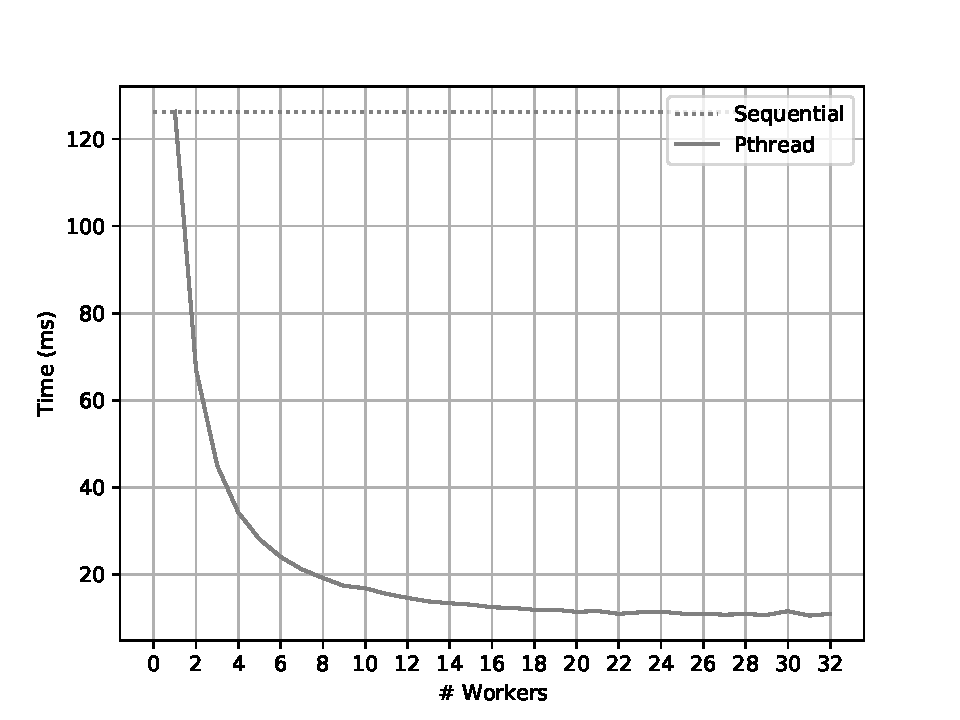
\includegraphics[width=\textwidth]{plots/pthread_performance_04_time.pdf}
    \end{minipage}
    \begin{minipage}{0.48\textwidth}
        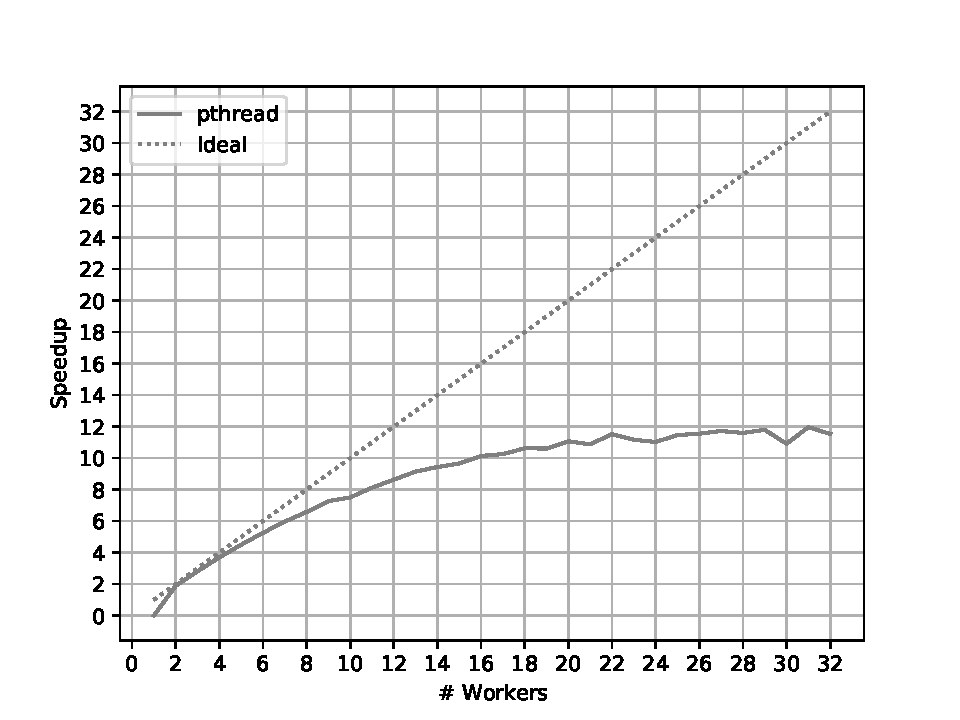
\includegraphics[width=\textwidth]{plots/pthread_speedup_04_time.pdf}
    \end{minipage}
    \caption{Performance and speedup of pthread version using 0.4 as value for p}
    \label{fig:pthread_04}
\end{figure}
\begin{figure}
    \centering
    \begin{minipage}{0.48\textwidth}
        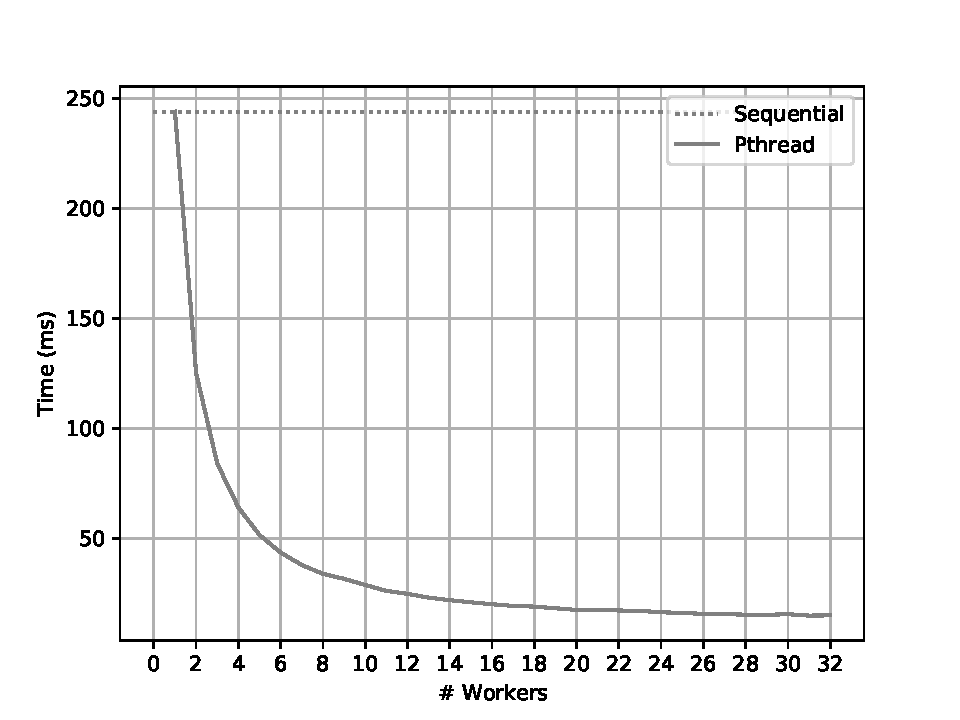
\includegraphics[width=\textwidth]{plots/pthread_performance_08_time.pdf}
    \end{minipage}
    \begin{minipage}{0.48\textwidth}
        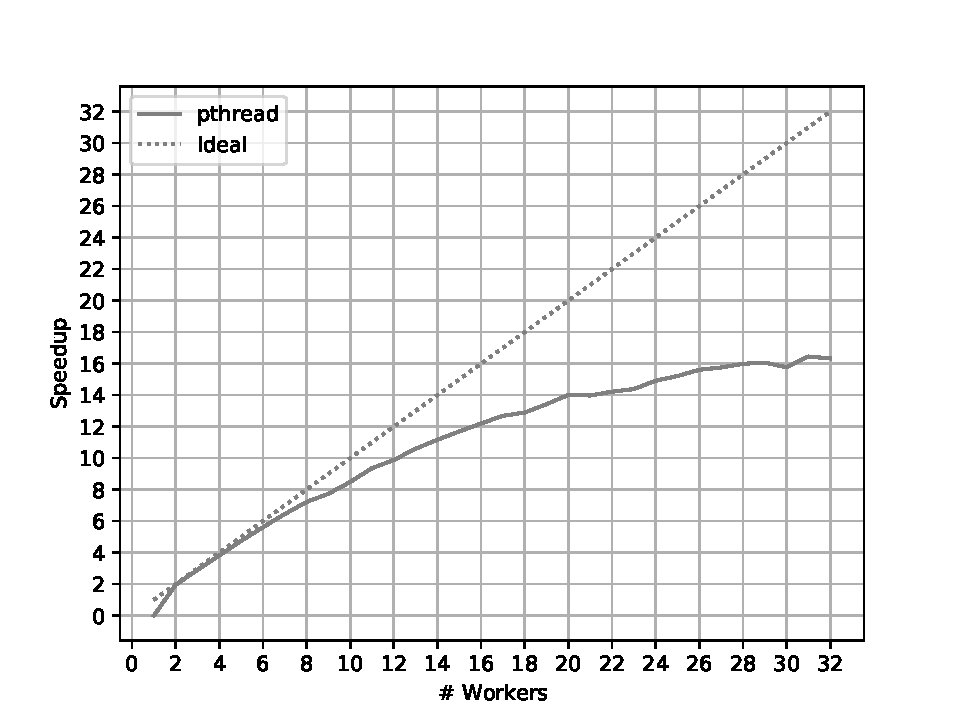
\includegraphics[width=\textwidth]{plots/pthread_speedup_08_time.pdf}
    \end{minipage}
    \caption{Performance and speedup of pthread version using 0.8 as value for p}
    \label{fig:pthread_08}
\end{figure}
\subsubsection{Overhead analysis}
TODO: scrivere
\subsubsection{Fastflow implementation}
TODO: scrivere

\begin{figure}
    \centering
    \begin{minipage}{0.48\textwidth}
        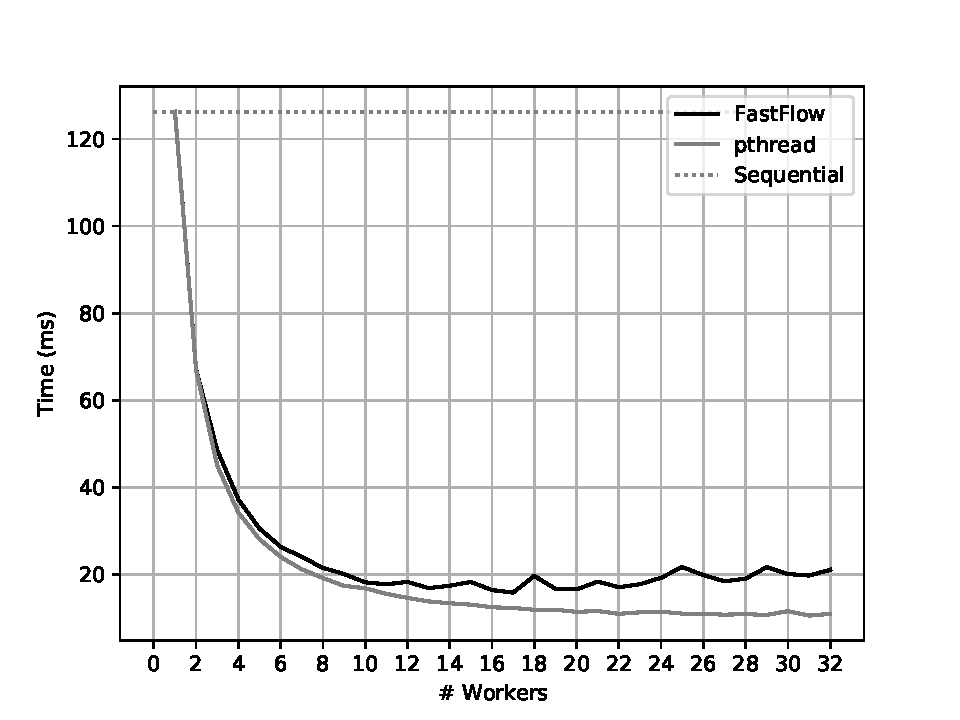
\includegraphics[width=\textwidth]{plots/fastflow_performance_04_time.pdf}
    \end{minipage}
    \begin{minipage}{0.48\textwidth}
        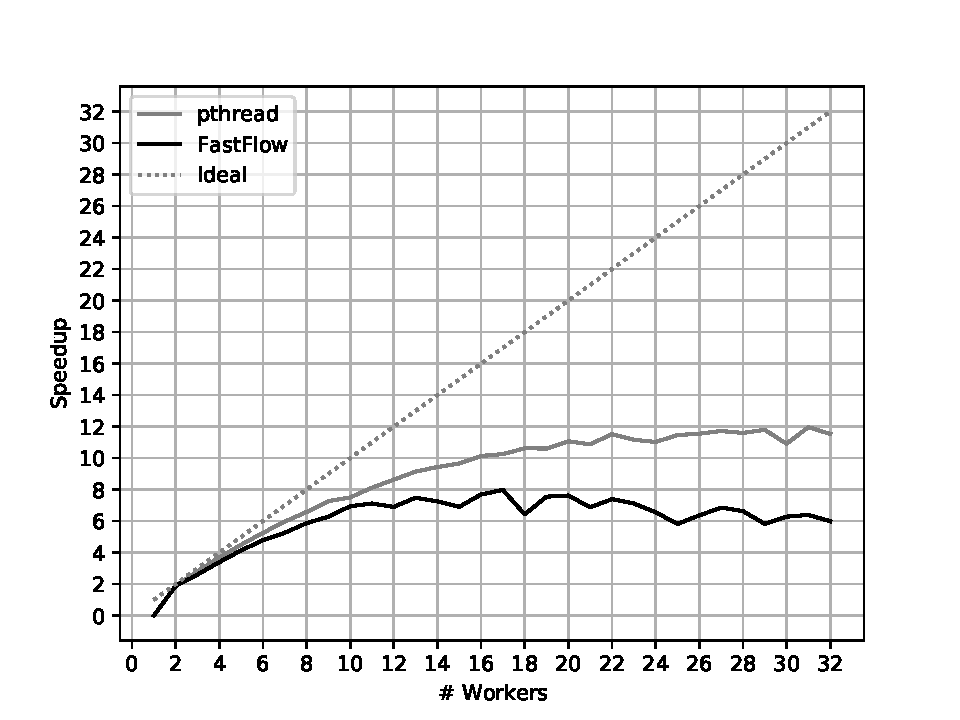
\includegraphics[width=\textwidth]{plots/fastflow_speedup_04_time.pdf}
    \end{minipage}
    \begin{minipage}{1\textwidth}
    \caption{Performance and speedup of FastFlow version using 0.4 as value for p}
    \label{fig:fastflow_04}
\end{minipage}
\end{figure}
\begin{figure}
    \centering
    \begin{minipage}{0.48\textwidth}
        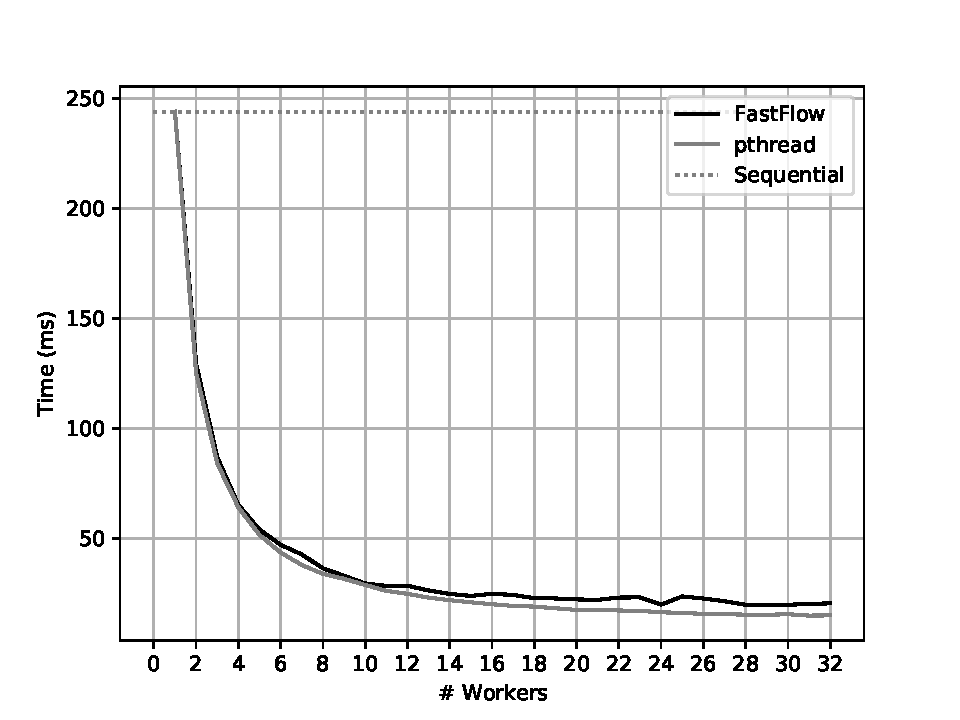
\includegraphics[width=\textwidth]{plots/fastflow_performance_08_time.pdf}
    \end{minipage}
    \begin{minipage}{0.48\textwidth}
        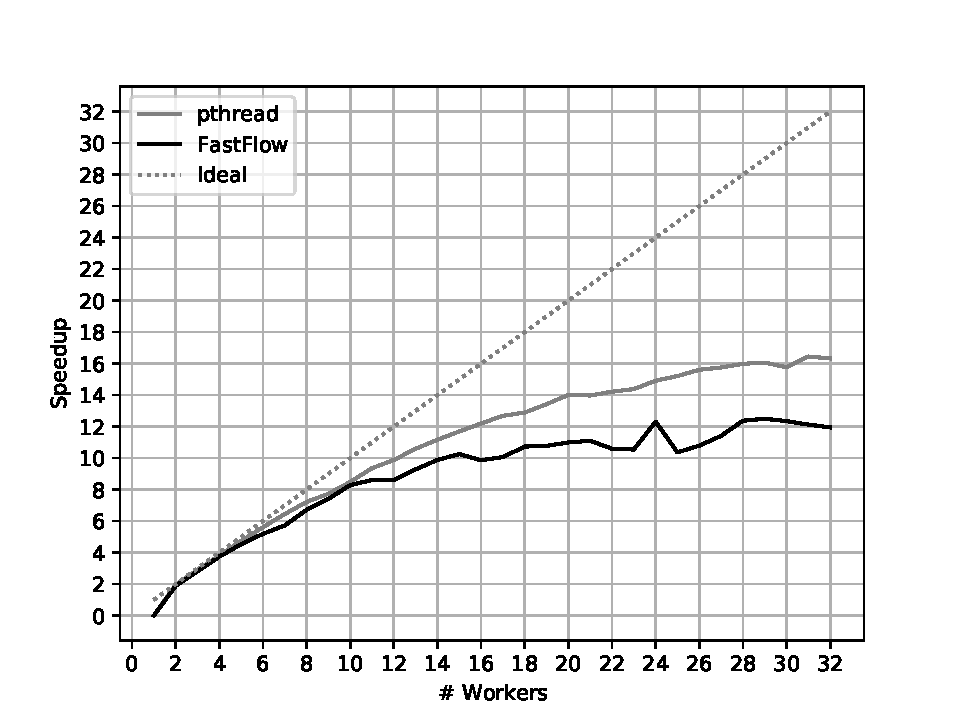
\includegraphics[width=\textwidth]{plots/fastflow_speedup_08_time.pdf}
    \end{minipage}
    \caption{Performance and speedup of FastFlow version using 0.8 as value for p}
    \label{fig:fastflow_08}
\end{figure}
\subsection{A real use case}
To end the section, a real case is shown, using as
 input a real network of $100000$ nodes and $\approx 500000$ edges. The 
 network was built as a network
  of interactions happened in the 
  month of october 
 2020 in the /r/politics subreddit. The nodes represent users who have 
 commented or written posts, while the edges from user 
 A to user B indicates that the former has posted a comment to the latter. 
 The results obtained are reported in terms of performance and speedup in 
 the Figure  \ref{fig:real-case}.

\begin{figure}
\centering
\begin{minipage}{0.48\textwidth}
    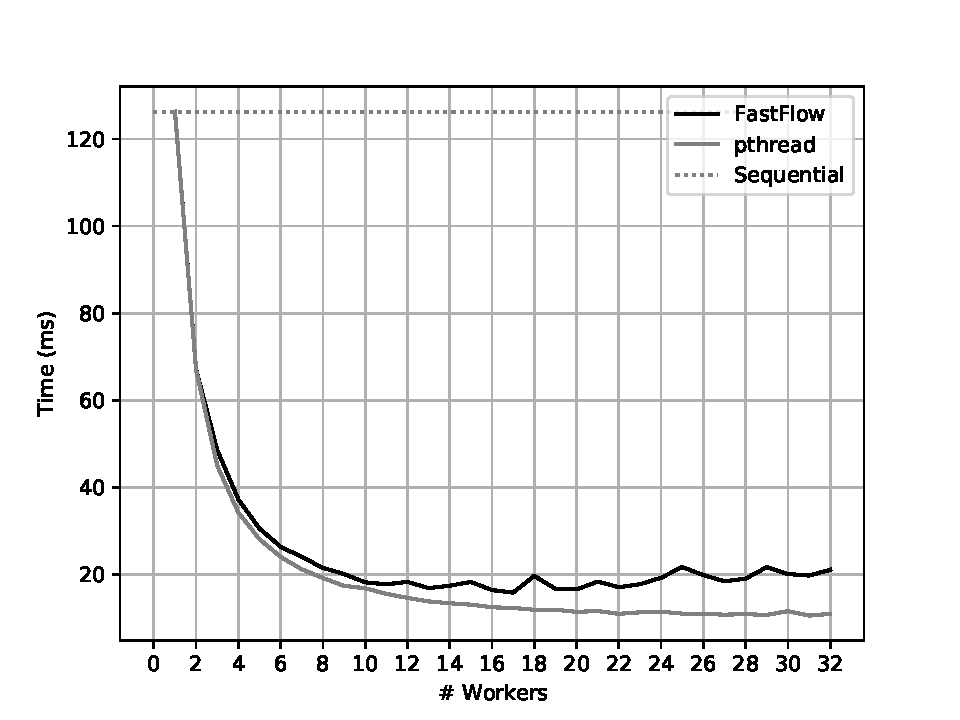
\includegraphics[width=\textwidth]{plots/fastflow_performance_04_time.pdf}
\end{minipage}
\begin{minipage}{0.48\textwidth}
    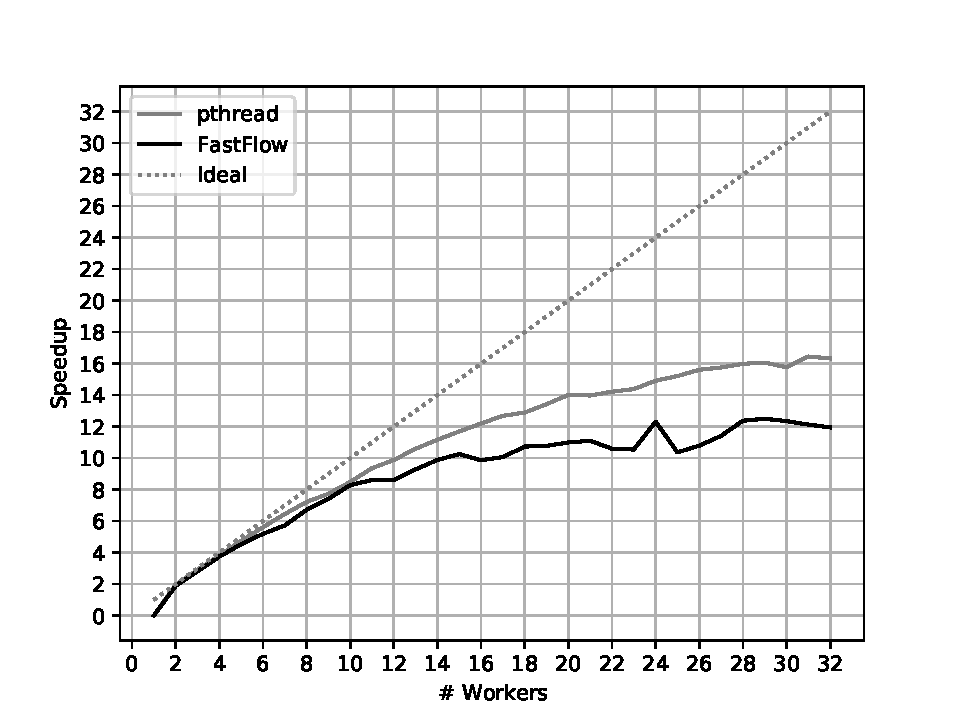
\includegraphics[width=\textwidth]{plots/fastflow_speedup_08_time.pdf}
\end{minipage}
\caption{Real use case speedup}
\label{fig:real-case}
\end{figure}

TODO: finire
\section{Conclusion}
The problem of BFS in parallel is very fascinating because the task itself looks easy, but considering the fact that it is strongly dependent on the input, is non trivial to design a solution that in general achieves good performances. Graphs, as it is known, have many statistical and topological properties, and an accurate analysis requires a lot of effort. The work presented here tries to analyze the performance of the proposed parallel solutions by varying some of the main properties of the graphs. The work focused more on some types of graphs, exposing reasoning  specifically on Erdos-Renyi graphs and real networks.
\\
In conclusion, the proposed solution achieves fair performance provided that we find sufficiently large frontiers and that the nodes of the next frontier are equally distributed in the neighborhoods of the current one. Two possible improvements can be applied: 
\begin{enumerate}
    \item The first one, is to handle the possibility that some frontiers may be very small, i`ntroducing a threshold on the number of nodes in the frontier under which the sequential version is used. 
    \item Another possible improvement to mitigate the problem of the distribution of nodes of the next frontier in the neighborhoods is the introduction of the concept of partial visit of a node. A simple way to implement it is to check at the time of insertion into the frontier how many neighbors the node has: if the number is above a certain threshold its visit is split into multiple chunks.
\end{enumerate}

\end{document}